\chapter{Work Breakdown Structure (WBS)}
In this chapter the tasks and work packages needed to perform the project will be specified. To do so, a WBS is developed.
\begin{enumerate}[label*=\arabic*.]
	\item PROJECT MANAGEMENT
	
	\begin{enumerate}[label*=\arabic*.]
		\item Development project management plan
		\item Monitoring of the project
		\begin{enumerate}[label*=\arabic*.]
			\item Meetings
			\item Task tracking and scheduling
		\end{enumerate}
		\item Annual reporting
		\item Project implementation of risk management
	\end{enumerate}
	
	\item QUALITY AND ADMINISTRATION
	\begin{enumerate}[label*=\arabic*.]
		\item Human Resources
		\begin{enumerate}[label*=\arabic*.]
			\item Employment of the necessary staff
			\item Human resources management
		\end{enumerate}
		\item Financial Plan
		\begin{enumerate}[label*=\arabic*.]
			\item Costs
			\begin{enumerate}[label*=\arabic*.]
				\item Fix costs
				\item Variable costs
			\end{enumerate}
			\item Funding
			\item Economic feasibility
			\item Evolution monitoring
			\item Additional and follow-up funding seek
		\end{enumerate}
		\item Documentation Management
		\begin{enumerate}[label*=\arabic*.]
			\item Guidelines preparation
			\item Document revision
			\item Document rectification
			\item Document approval
		\end{enumerate}
		\item Periodic Monitoring
	\end{enumerate}

	\item STATE OF THE ART
	
	\begin{enumerate}[label*=\arabic*.]
		\item Payloads
		\begin{enumerate}[label*=\arabic*.]
			\item Search for current space applications
			\item Requirements definition
		\end{enumerate}
		\item Modular System
		\begin{enumerate}[label*=\arabic*.]
			\item Search for current modular systems with space applications
			\item Requirements definition
		\end{enumerate}
		\item Urban Development Applications with Space Technologies
		\begin{enumerate}[label*=\arabic*.]
			\item Search for current space applications
			\begin{enumerate}[label*=\arabic*.]
				\item Weather forecast
				\item Urban planning (3D models)
				\item Greenhouse emissions reduction (pollution)
			\end{enumerate}
			\item Requirements definition
		\end{enumerate}
	\end{enumerate}
	
	\item PRODUCT DEVELOPMENT
	
	\begin{enumerate}[label*=\arabic*.]
		\item Preliminary Design
		\begin{enumerate}[label*=\arabic*.]
			\item Payloads
			\begin{enumerate}[label*=\arabic*.]
				\item Research
				\item Development
			\end{enumerate}
			\item Modular system
			\begin{enumerate}[label*=\arabic*.]
				\item Development of physical framework for sensor blocks
				\item Development of systems interaction and applications
				\item Development of sensors data fusion software
				\item Definition of SATCOM applications domains
			\end{enumerate}
			\item Interaction platform
			\begin{enumerate}[label*=\arabic*.]
				\item Implement web-based servers for sharing sensors data
				\item Implement processing algorithms based on applications
%				\begin{enumerate}[label*=\arabic*.]
%					\item Terrain mapping
%					\item Greenhouse gases emission
%					\item Weather forecast
%				\end{enumerate}
				\item Pre-design a full services stakeholders platform 
			\end{enumerate}
		\end{enumerate}
		\item Final design
		\begin{enumerate}[label*=\arabic*.]
			\item Payloads 
			\begin{enumerate}[label*=\arabic*.]
				\item Sensors final design
				\item Sensors final technical specifications
			\end{enumerate}
			\item Modular System
			\begin{enumerate}[label*=\arabic*.]
				\item Modular system final design
				\item Sensors data fusion software final design
				\item Modular system's final technical specifications
			\end{enumerate}
			\item Interaction Platform
			\begin{enumerate}[label*=\arabic*.]
				\item Web based servers for data sharing final implementation
				\item Processing algorithms based on applications final design
				\item Full services stakeholders platform implementation
				\item Final technical specifications
			\end{enumerate}
		\end{enumerate}
	\end{enumerate}
	
	\item SIMULATION, TESTING, VALIDATION AND QUALITY
	
	\begin{enumerate}[label*=\arabic*.]
		\item Technology Demonstrator Prototype Manufacturing
		\begin{enumerate}[label*=\arabic*.]
			\item Manufacturing of payload sensors
			\item Manufacturing of modular system
			\item Implementation of interaction platform
		\end{enumerate}
		\item Payload Validation
		\item Modular System Validation
		\item Interaction Platform Validation
		\item Full System Prototype Validation
		\item Quality of the Product
	\end{enumerate}
	
	\item BUSINESS PLANNING AND EXPLOITATION OF RESULTS
	
	\begin{enumerate}[label*=\arabic*.]
		\item Market Approach
		\begin{enumerate}[label*=\arabic*.]
			\item Study of stakeholders
			\item Procurement conditions negotiation
			\item Resources purchase	
		\end{enumerate}
		\item Exploitation and Business Plans
	\end{enumerate}
	
	\item COMMUNICATION AND DISSEMINATION STRATEGIES
	
	\begin{enumerate}[label*=\arabic*.]
		\item Dissemination and Communication Plan
		\item On-line Dissemination/Communication Activities
		\begin{enumerate}[label*=\arabic*.]
			\item Web site development
			\item Social media management
		\end{enumerate}
		\item Off-line Dissemination/Communication Activities
		\begin{enumerate}[label*=\arabic*.]
			\item Conferences
			\item Meetings
		\end{enumerate}
		\item Production of Dissemination Materials
		\begin{enumerate}[label*=\arabic*.]
			\item Technology demonstrators
			\item Audio visual material production
		\end{enumerate}
	\end{enumerate}
	
\end{enumerate}

In the following pages this WBS will be exposed in a more graphical manner. In order to see it properly it has been split into different blocks. \\
\vspace{10mm}

\begin{figure}[H]
	\centering
	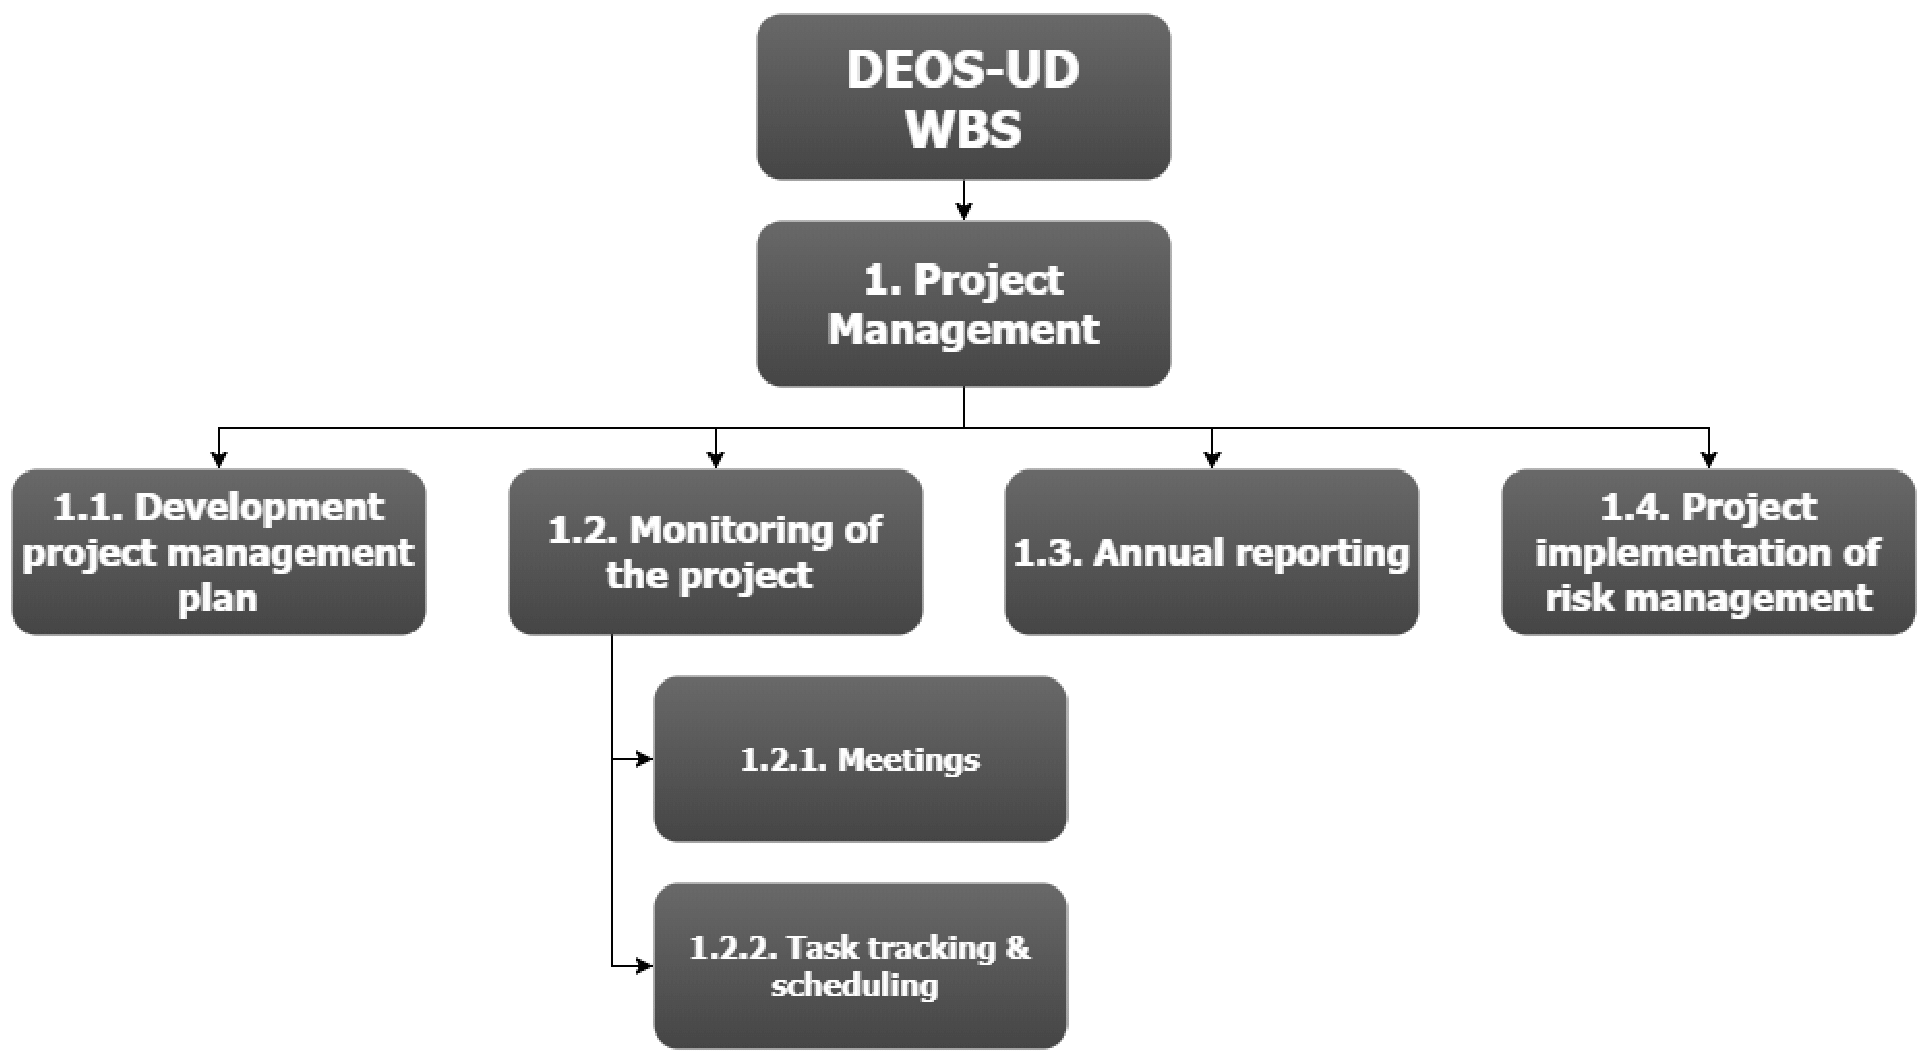
\includegraphics[width=\textwidth]{./sections/2.WBS/WBS_Section1}
	\caption[Project management breakdown diagram]{Project management breakdown diagram.}
	\label{fig:WBS_Section1}
\end{figure}

\begin{figure}[H]
	\centering
	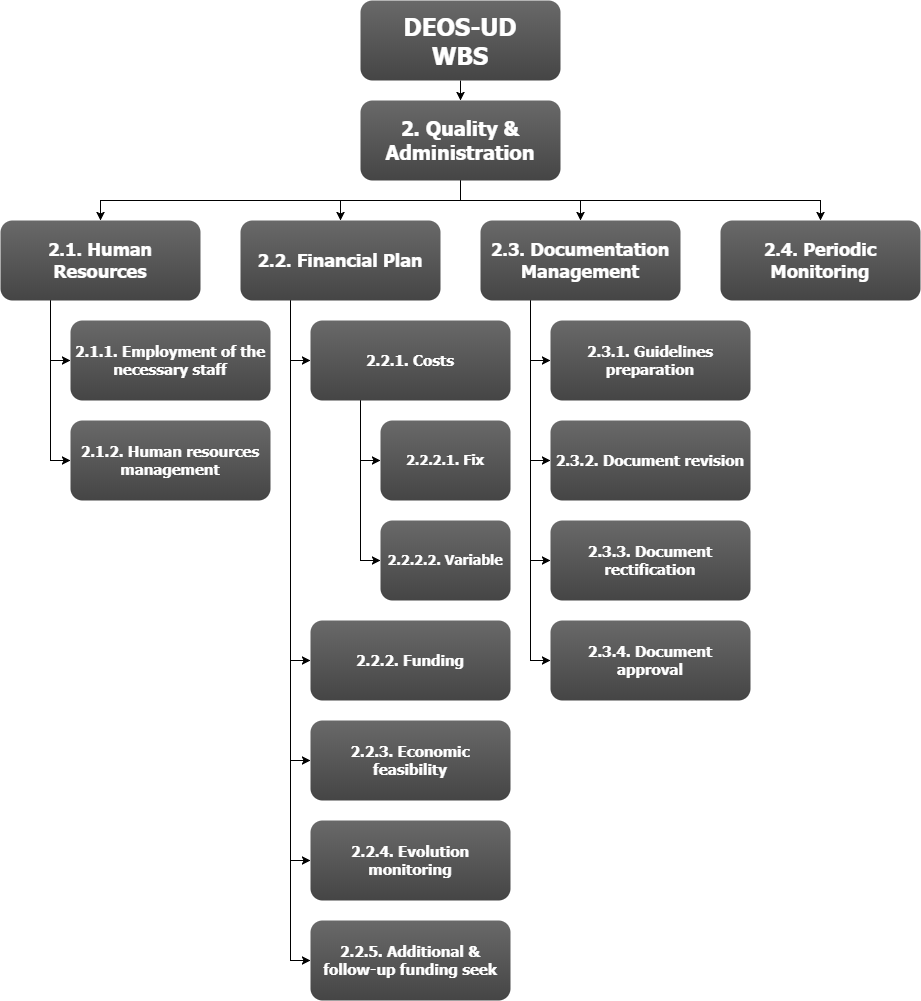
\includegraphics[width=\textwidth]{./sections/2.WBS/WBS_Section2}
	\caption[Quality and administration breakdown diagram]{Quality and administration breakdown diagram.}
	\label{fig:WBS_Section2}
\end{figure}

\begin{figure}[H]
	\centering
	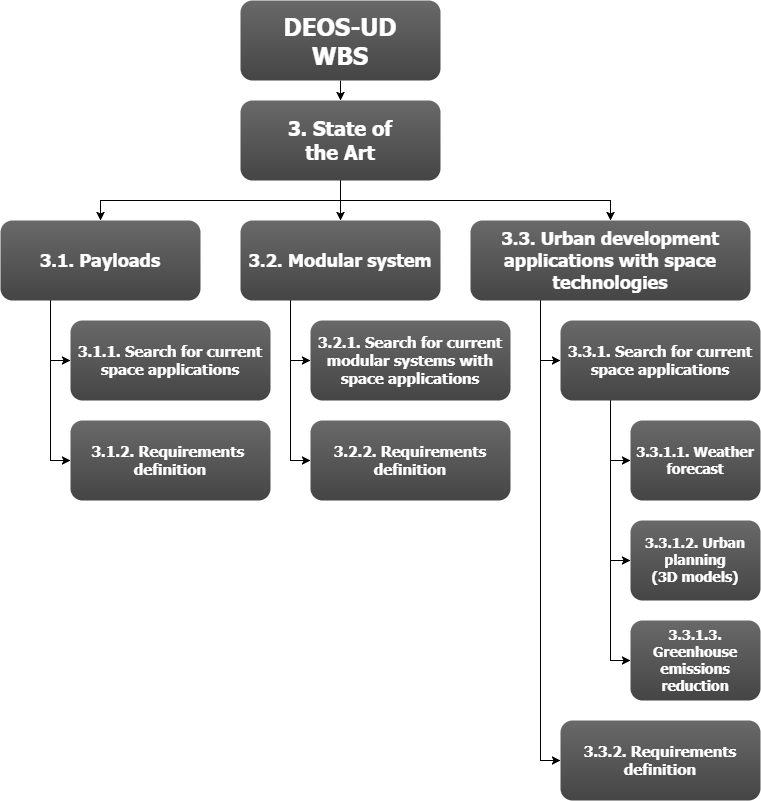
\includegraphics[width=\textwidth]{./sections/2.WBS/WBS_Section3}
	\caption[State of the art breakdown diagram]{State of the art breakdown diagram.}
	\label{fig:WBS_Section3}
\end{figure}

\begin{landscape}\tiny

\vspace*{\fill}
\begin{figure}[H]
	\centering
	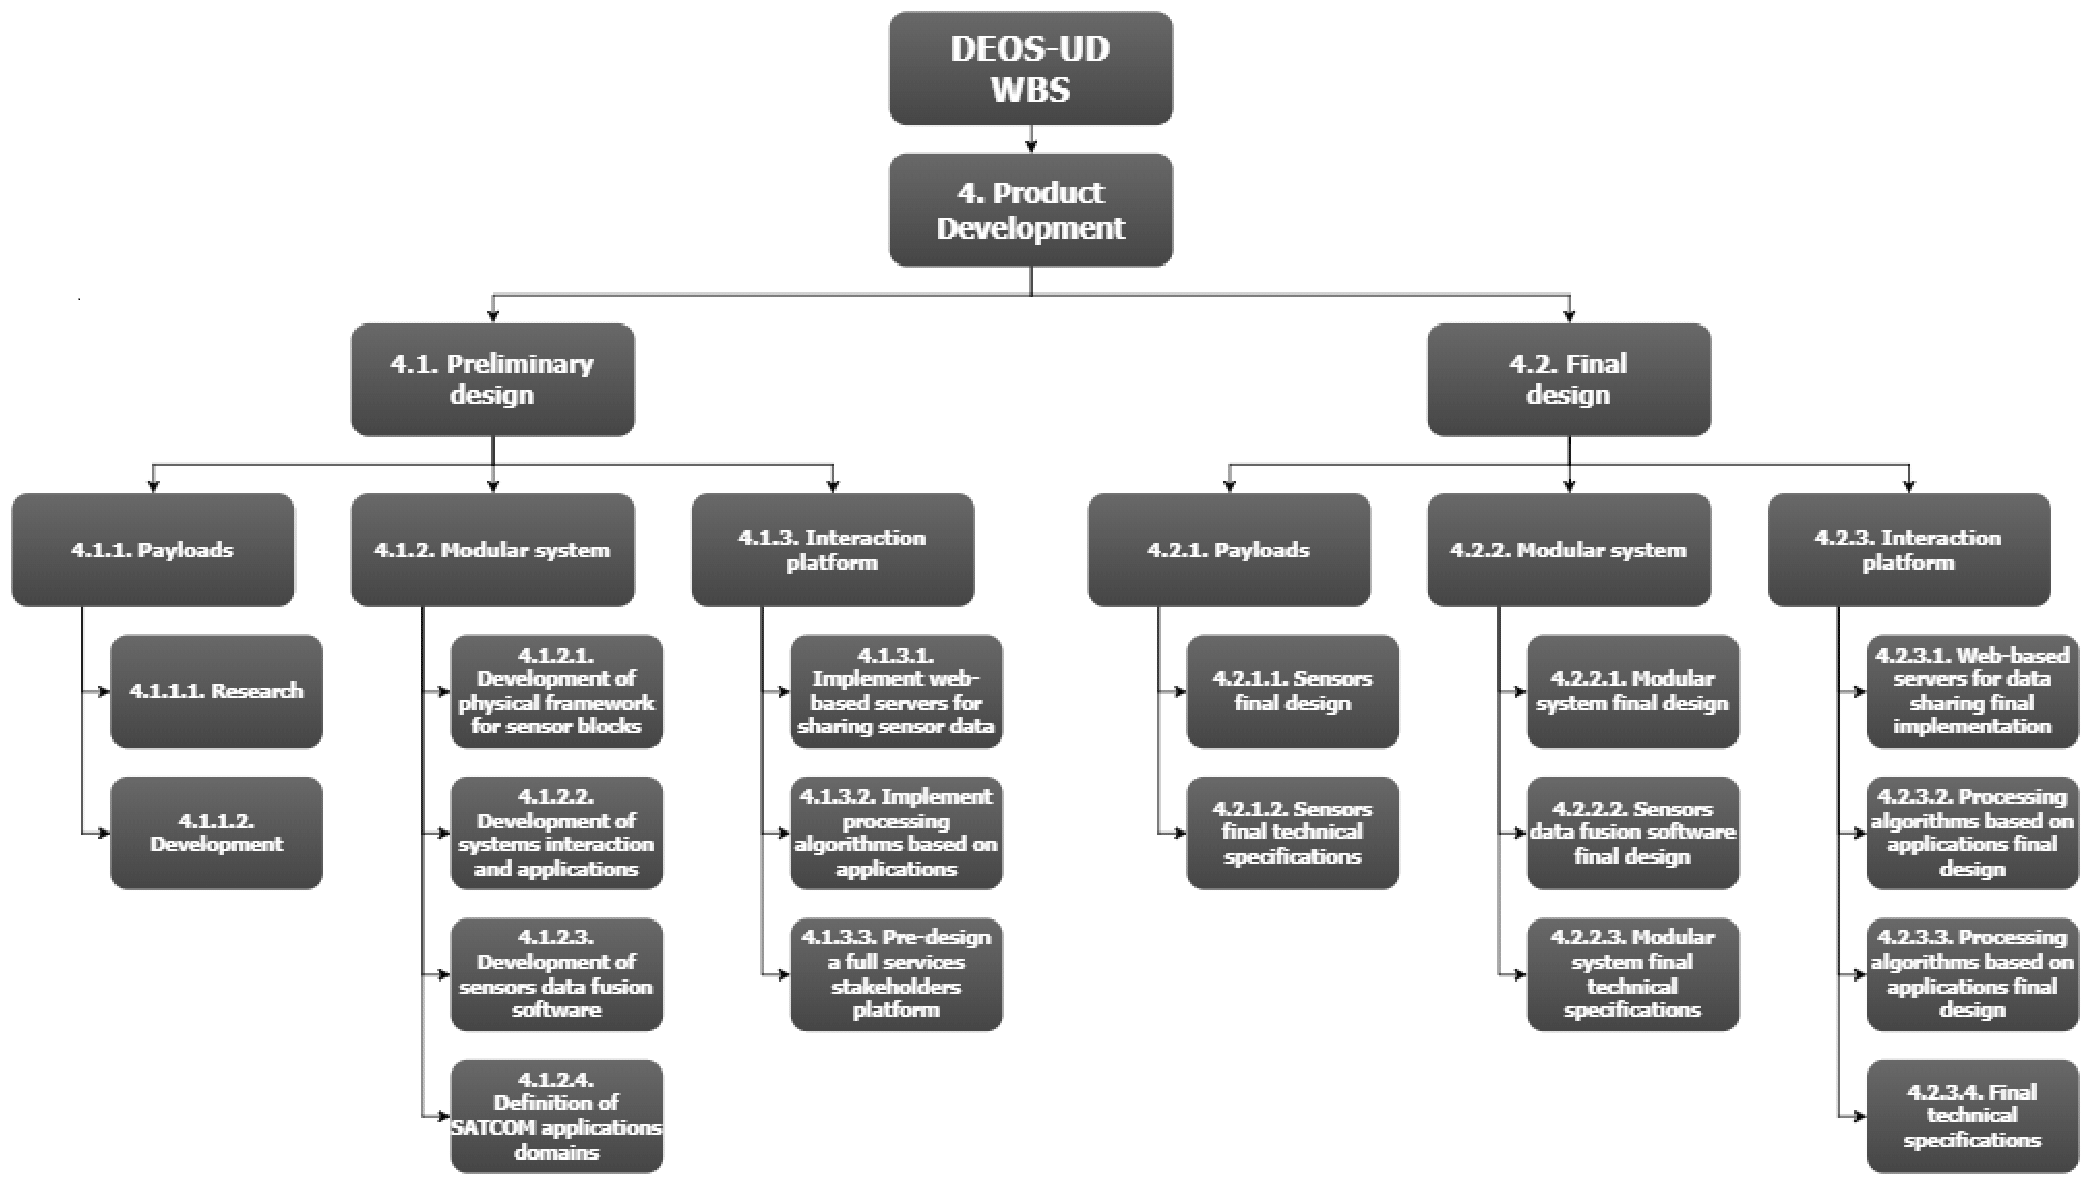
\includegraphics[width=1.5\textwidth]{./sections/2.WBS/WBS_Section4}
	\caption[Product development breakdown diagram]{Product development breakdown diagram.}
	\label{fig:WBS_Section4}
\end{figure}
\vspace*{\fill}

\end{landscape}


\begin{landscape}\tiny

\vspace*{\fill}
\begin{figure}[H]
	\centering
	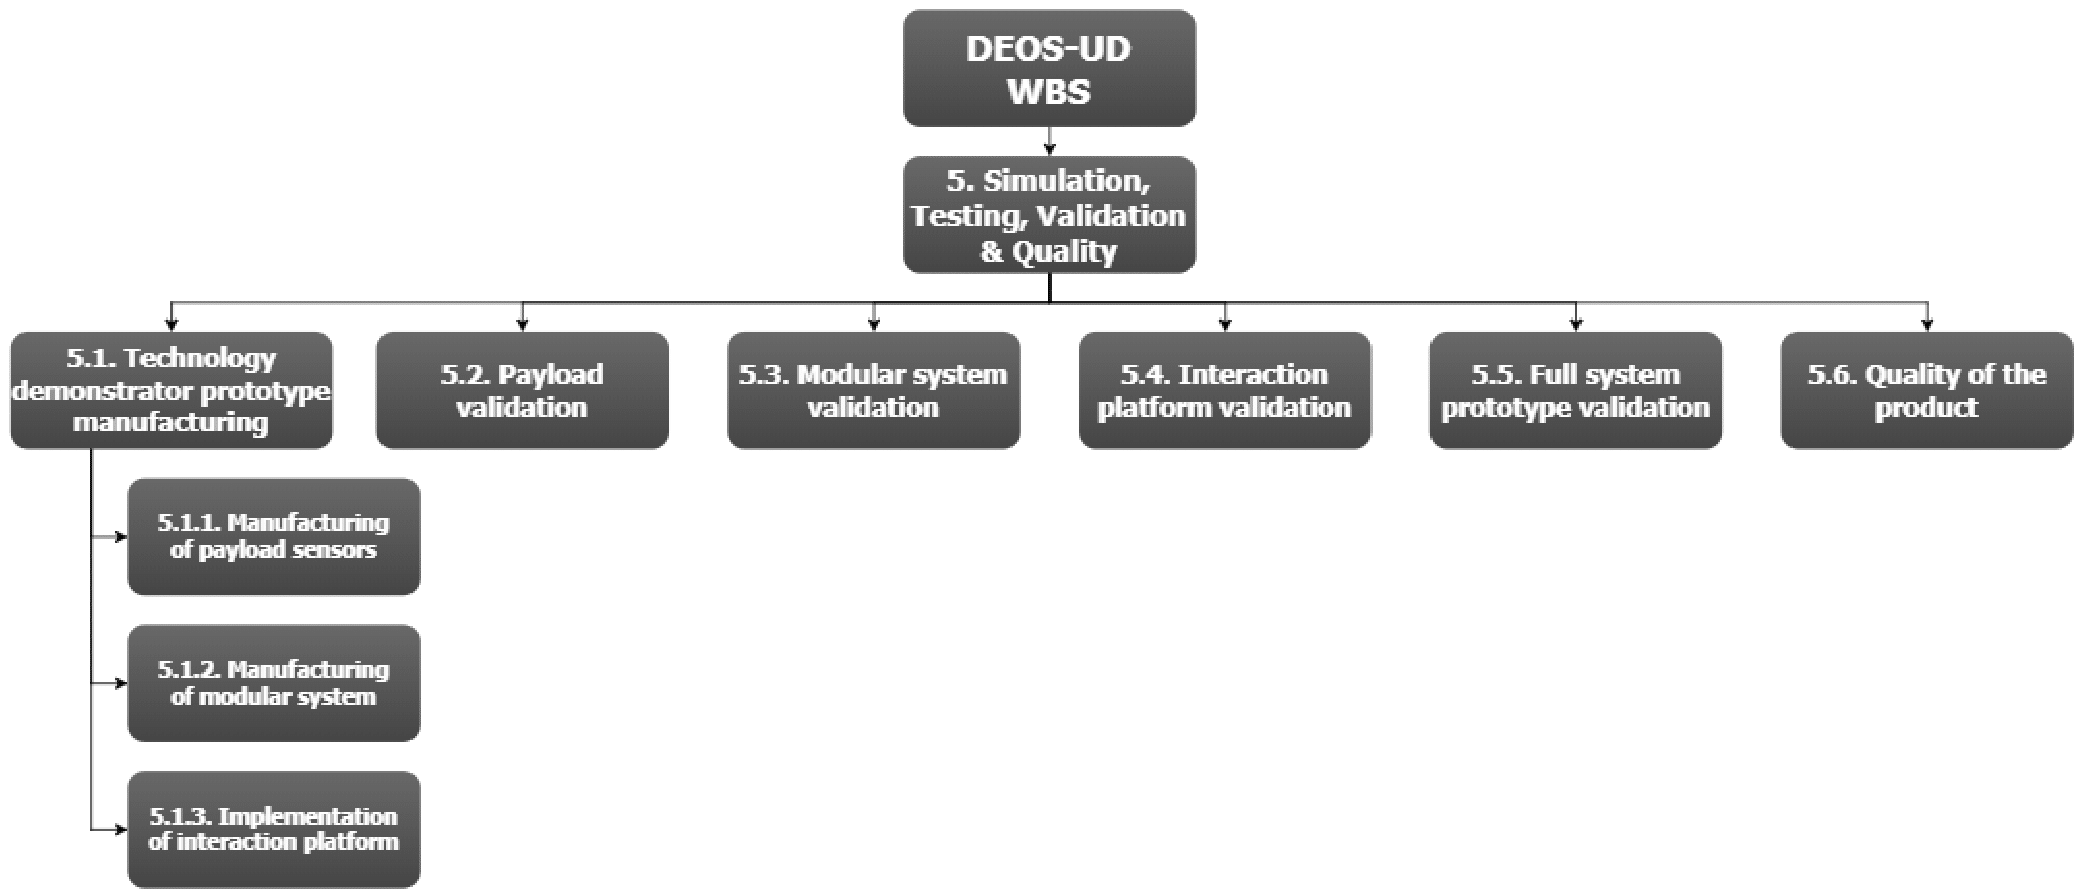
\includegraphics[width=1.5\textwidth]{./sections/2.WBS/WBS_Section5}
	\caption[Simulation, testing, validation and quality breakdown diagram]{Simulation, testing, validation and quality breakdown diagram.}
	\label{fig:WBS_Section5}
\end{figure}
\vspace*{\fill}

\end{landscape}

\vspace*{\fill}
\begin{figure}[H]
	\centering
	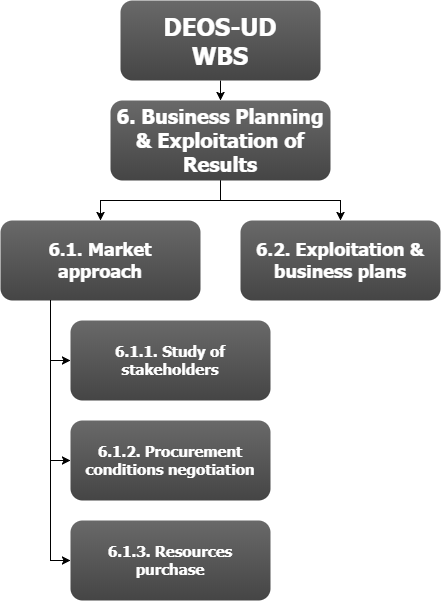
\includegraphics[height=13cm,keepaspectratio]{./sections/2.WBS/WBS_Section6}
	\caption[Business planning and exploitation of results breakdown diagram]{Business planning and exploitation of results breakdown diagram.}
	\label{fig:WBS_Section6}
\end{figure}
\vspace*{\fill}

\begin{landscape}\tiny

\vspace*{\fill}
\begin{figure}[H]
	\centering
	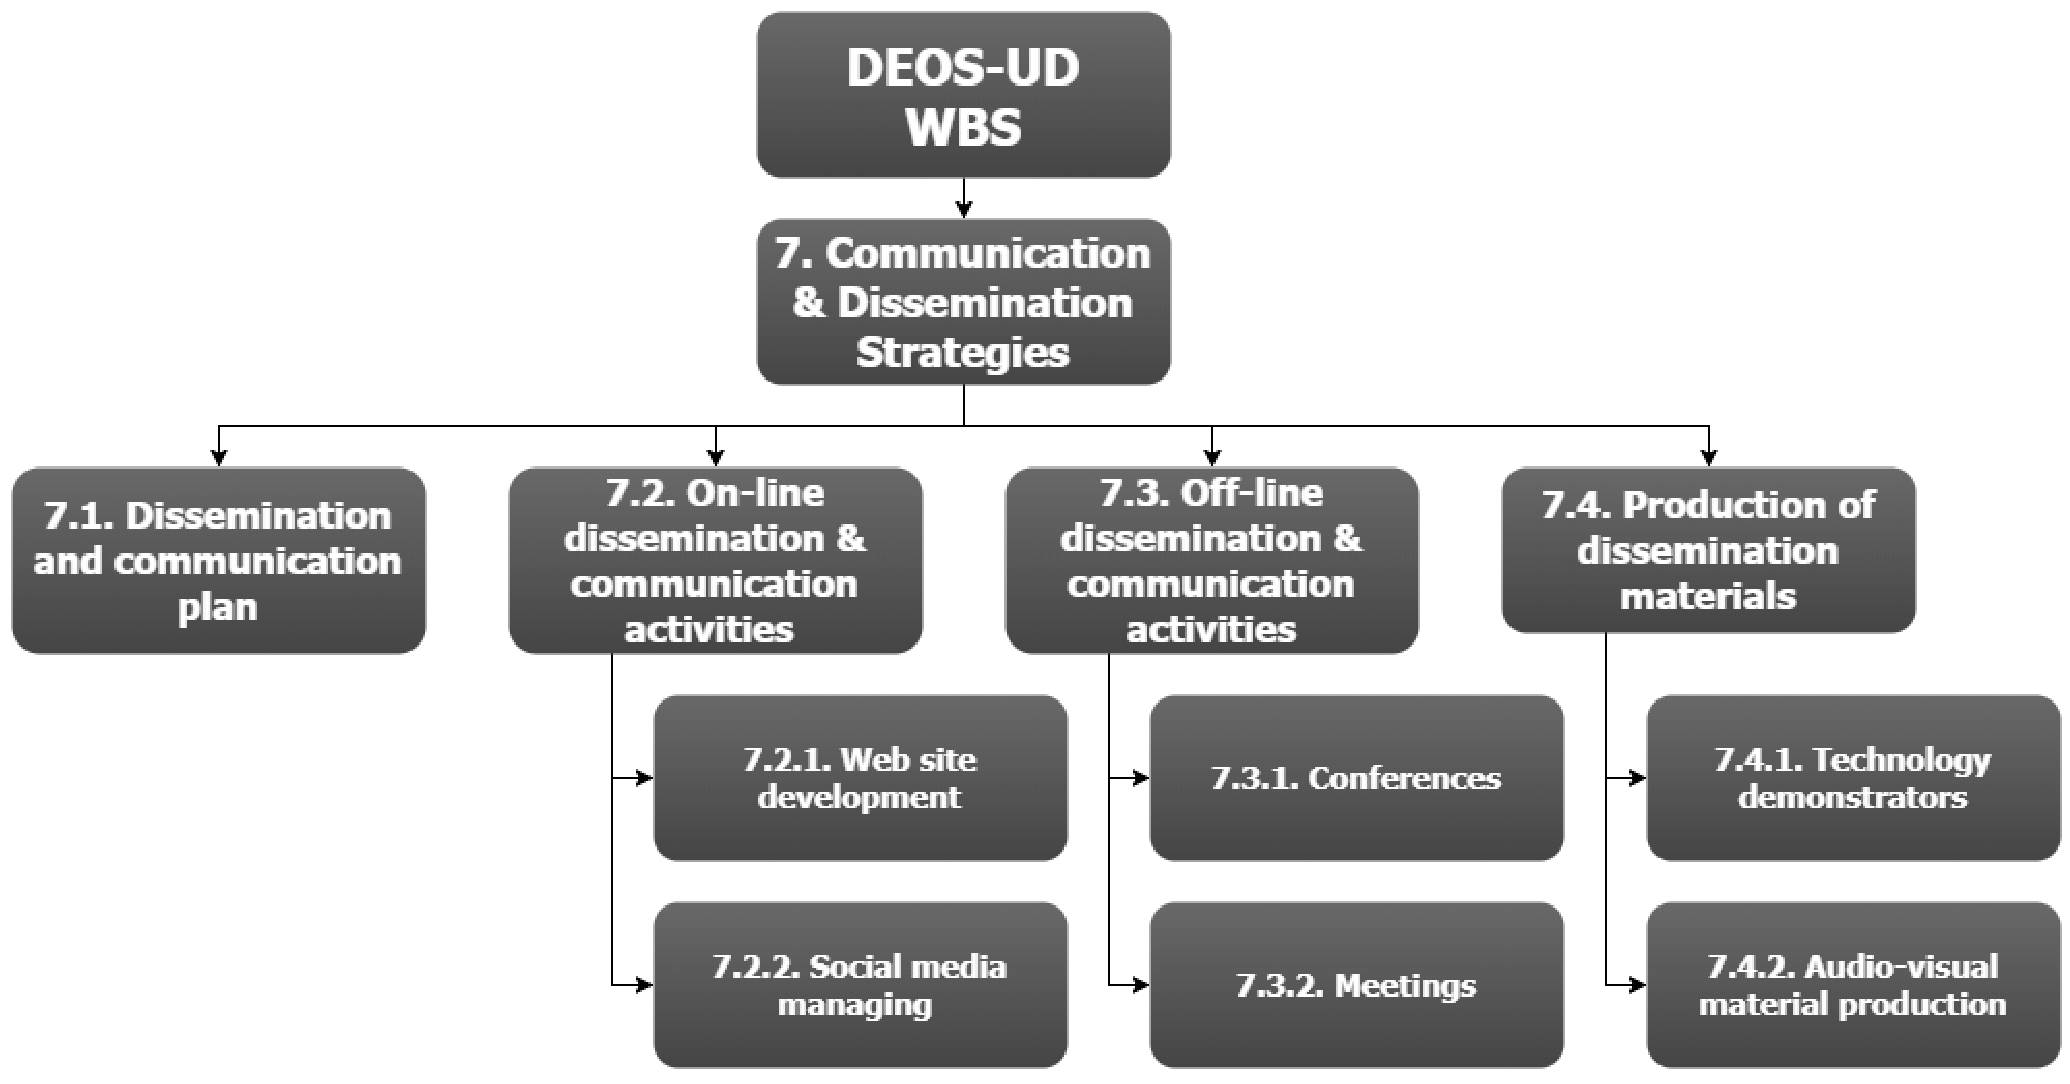
\includegraphics[width=1.3\textwidth]{./sections/2.WBS/WBS_Section7}
	\caption[Communication and dissemination strategies breakdown diagram]{Communication and dissemination strategies breakdown diagram.}
	\label{fig:WBS_Section7}
\end{figure}
\vspace*{\fill}

\end{landscape}


\section{Activity list}

\begin{longtable}[H]{l >{\raggedright\arraybackslash}p{4cm} p{8cm}}
	
	\toprule[2pt]
	
	\textbf{WBS-ID} &  \textbf{Activity}  & \textbf{Description of Work} \\
	
	\midrule [1.5pt]
	\endhead
	
	1. & Project Management & All activities related to the management of the project fall under this activity.\vspace{0.2cm} \\
	
	\midrule
	
	1.1. & Development of the project management plan &Elaboration of all the documentation that states the strategy of the management and organization of the project through its duration.\vspace{0.2cm} \\
	
	\midrule
	
	1.2. & Monitoring of the project & Control of the progress of each activity of the project.\vspace{0.2cm} \\
	
	\midrule
	
	1.2.1. & Meetings & Gathering of the members of the project to inform each other of the progress.\vspace{0.2cm} \\
	
	\midrule
	
	1.2.2. & Task tracking and scheduling & Tracking of the active tasks and scheduling.\vspace{0.2cm} \\
	
	\midrule
	
	1.3. & Annual reporting & Every year that the project lasts will call for the elaboration of an internal report with the aim of keeping up to date with the progress done.\vspace{0.2cm} \\
	
	\midrule
	
	1.4. & Project implementation of risk management & Study of all the potential risks and how will they be managed so that their affectation to the project stays to a minimum.\vspace{0.2cm} \\
	
	\midrule
	
	2. & Quality and Administration & Activities related to the administrative aspects of the project and to assure the quality of all the documents presented.\vspace{0.2cm} \\
	
	\midrule
	
	2.1. & Human resources & Administration of all the employees needed to fulfill the different tasks of the project.\vspace{0.2cm} \\
	
	\midrule
	
	2.1.1. & Employment of the necessary staff & Definition of the number of employees necessary.\vspace{0.2cm} \\
	
	\midrule
	
	2.1.2. & Human resources management & Administration of all the employees needed to fulfill the different tasks of the project.\vspace{0.2cm} \\
	
	\midrule
	
	2.2. & Financial plan & Lay down of all the planned costs of the project, the funding expected from the various sources, a study on the economic feasibility of the project and a plan for additional funding search.\vspace{0.2cm} \\
	
	\midrule
	
	2.2.1. & Costs & Lay down of all the planned costs of the project.\vspace{0.2cm} \\
	
	\midrule
	
	2.2.1.1. & Fix costs & Lay down of all the fix costs of the project.\vspace{0.2cm} \\
	
	\midrule
	
	2.2.1.2. & Variable costs & Lay down of all the variable costs of the project.\vspace{0.2cm} \\
	
	\midrule
	
	2.2.2. & Funding & Lay down of all the expected funding of the project.\vspace{0.2cm} \\
	
	\midrule
	
	2.2.3. & Economic feasibility & Study on the economic feasibility of the project.\vspace{0.2cm} \\
	
	\midrule
	
	2.2.4. & Evolution monitoring & Monitoring of the evolution of the project finances.\vspace{0.2cm} \\
	
	\midrule
	
	2.2.5. & Additional and follow-up funding seek & Search for the additional funding for the project.\vspace{0.2cm} \\
	
	\midrule
	
	2.3. & Documentation management & The quality of the documents that have to be delivered through all the duration of the project is guaranteed in this activity by establishing guidelines for the redaction of all the documents, their revision and posterior rectification and final approval.\vspace{0.2cm} \\
	
	\midrule
	
	2.3.1. & Guidelines preparation & Establishment of the guidelines for the relation of all documents.\vspace{0.2cm} \\
	
	\midrule
	
	2.3.2. & Documented revision & Revision of all the documents of the project.\vspace{0.2cm} \\
	
	\midrule
	
	2.3.3. & Document rectification & Rectification of the documents that do not meet the project requirements.\vspace{0.2cm} \\
	
	\midrule
	
	2.3.4. & Document approval & Approval of the reviewed and rectified documents.\vspace{0.2cm} \\
	
	\midrule
	
	2.4. & Periodic monitoring & To ensure the quality of the project, a periodic monitoring of all the activities will be carried out.\vspace{0.2cm} \\
	
	\midrule
	
	3. & State of the Art & Before starting the design and research it is key to have an accurate vision of the actual state of the technology that is going to be developed.\vspace{0.2cm} \\
	
	\midrule
	
	3.1. & Payloads & For each of the sensors that are planned to be improved there is a search of the current space applications, that helps to define the requirements for these sensors.\vspace{0.2cm} \\
	
	\midrule
	
	3.1.1. & Search for current space applications & Search for the current space applications.\vspace{0.2cm} \\
	
	\midrule
	
	3.1.2 & Requirements definition & Definition of the requirements for the the sensors.\vspace{0.2cm} \\
	
	\midrule
	
	3.2. & Modular system & For the modular system where each sensor will be mounted on there will be a search of current similar systems in space applications and the definition of the requirements for the one developed in this project.\vspace{0.2cm} \\
	
	\midrule
	
	3.2.1. & Search for the current modular systems with space applications & Search for the current modular systems with space applications.\vspace{0.2cm} \\
	
	\midrule
	
	3.2.2. & Requirements definition & Definition of the requirements for modular system developed in this project.\vspace{0.2cm} \\
	
	\midrule
	
	3.3. & Urban development applications & The search for current applications similar to those that want to be implemented with this project has to be carried out, in the weather forecast area, the urban planning area and the greenhouse emissions reduction area, thus defining the requirements for the applications.\vspace{0.2cm} \\
	
	\midrule
	
	3.3.1.1. & Weather forecast & Search for current applications similiar to those that want to be implemented with this project in the weather forecast area.\vspace{0.2cm} \\
	
	\midrule
	
	3.3.1.2. & Urban planning (3D models) & Search for the current applications to those that want to be implemented with this project in the urban planning area.\vspace{0.2cm} \\
	
	\midrule
	
	3.3.1.3. & Greenhouse emissions reduction (pollution) & Search for the current applications to those that want to be implemented with this project in the greenhouse emissions reduction area.\vspace{0.2cm} \\
	
	\midrule
	
	3.3.2. & Requirements definition & Definition of the requirements fotr the applications.\vspace{0.2cm} \\
	
	\midrule
	
	4. & Product development & All the phases of the development of the product are included in this activity, from the research up to the final technical specifications.\vspace{0.2cm} \\
	
	\midrule
	
	4.1. & Preliminary design & This first phase of the development is meant to include all the research and definition of the initial parameters of the different components.\vspace{0.2cm} \\
	
	\midrule
	
	4.1.1. & Payloads' preliminary design & The research and initial development of each sensor that is intended to improve is carried out in this phase.\vspace{0.2cm} \\
	
	\midrule
	
	4.1.1.1. & Research & Research for the payloads preliminary design.\vspace{0.2cm} \\
	
	\midrule
	
	4.1.1.2. & Development & Development of the payloads preliminary design.\vspace{0.2cm} \\
	
	\midrule
	
	4.1.2. & Modular system's preliminary design & Includes the initial development of the physical framework for sensor blocks, of the systems' interaction and applications, of the sensors' data fusion software and the definition of the satellite communications applications domains.\vspace{0.2cm} \\
	
	\midrule
	
	4.1.2.1. & Development of physical framework for sensor block & Modular system preliminary design and development of physiscal framework for sensor block.\vspace{0.2cm} \\
	
	\midrule
	
	4.1.2.2. & Development of systems interaction and applications & Modular system preliminary design and development of systems interactions and applications.\vspace{0.2cm} \\
	
	\midrule
	
	4.1.2.3. & Development of sensors data fusion software & Modular system preliminary design and development of sensor data fusion software.\vspace{0.2cm} \\
	
	\midrule
	
	4.1.2.4. & Definition of SATCOM applications domains & Modular system preliminary design and definition of SATCOM application domains.\vspace{0.2cm} \\
	
	\midrule
	
	4.1.3. & Interaction platform's preliminary design & Implementation of the web-based servers for sharing sensor's data, of the processing algorithms based on applications and the pre-design of a full services stakeholders platform.\vspace{0.2cm} \\
	
	\midrule
	
	4.1.3.1. & Implement web-bases servers for sharing sensors data & Preliminary design of the interaction platform. Implement web-based servers for sharing sensors data.\vspace{0.2cm} \\
	
	\midrule
	
	4.1.3.2. & Implement processing algorithms based on applications & Preliminary design of the interaction platform. Implement processing algorithms based on applications.\vspace{0.2cm} \\
	
	\midrule
	
	4.1.3.3. & Pre-design a full services stakeholders platform & Pre-design of interaction platform.\vspace{0.2cm} \\
	
	\midrule
	
	4.2. & Final design & This final phase of the product's development will define the final technical specifications of each part of the product.\vspace{0.2cm} \\
	
	\midrule
	
	4.2.1. & Payloads' final design & The design of each sensor is complete and its final technical specifications are defined.\vspace{0.2cm} \\
	
	\midrule
	
	4.2.1.1. & Sensor final design & Final design of the payload sensor.\vspace{0.2cm} \\
	
	\midrule
	
	4.2.1.2. & Sensor final technical specifications & Final decision of the technical specifications of the payload sensor.\vspace{0.2cm} \\
	
	\midrule
	
	4.2.2. & Modular system & The design of the modular system and the sensors' data fusion software is complete and their final technical specifications are defined.\vspace{0.2cm} \\
	
	\midrule
	
	4.2.2.1. & Modular system's final design & Final design of the modular system.\vspace{0.2cm} \\
	
	\midrule
	
	4.2.2.2. & Sensor data fusion software final design  & Final design of the modular system, specifically of the sensor data fusion software.\vspace{0.2cm} \\
	
	\midrule
	
	4.2.2.3. & Modular system final technical specifications & Final decision of technical specifications of the modular system.\vspace{0.2cm} \\
	
	\midrule
	
	4.2.3. & Interaction platform's final design & The design of the interaction platform is complete, including the web based servers for data sharing, the processing algorithms based on applications and the full services stakeholders platform, and their final technical specifications are defined.\vspace{0.2cm} \\
	
	\midrule
	
	4.2.3.1. & Web based servers for data sharing final implementation & Final design and implementations of the interaction platform, specifically the web servers for data sharing.\vspace{0.2cm} \\
	
	\midrule
	
	4.2.3.2. & Processing algorithms based on applications final design & Final design and implementation of the interaction platfomr, specifically the processing algorithms.\vspace{0.2cm} \\
	
	\midrule
	
	4.2.3.3. & Full service stakeholders platform implementation & Final design and implementation of the itneraction platform.\vspace{0.2cm} \\
	
	\midrule
	
	4.2.3.4. & Final technical specifications & Decision of the final technical specifications of the interaction (stakeholders) platform.\vspace{0.2cm} \\
	
	\midrule
	
	5. & Simulation, testing, validation and quality & Activities regarding the simulation, testing, validation and quality control of the final product are included in this task.\vspace{0.2cm} \\
	
	\midrule
	
	5.1. & Technology demonstrator prototype manufacturing & Manufacturing of the prototype of the product, including all its subsystems (payload sensors, modular system and interaction platform), in order to be tested in the following activities.\vspace{0.2cm} \\
	
	\midrule
	
	5.1.1. & Manufacturing of payload sensors. & Manufacturing of the sensors of the prototype, in order to be tested in the following activities.\vspace{0.2cm} \\
	
	\midrule
	
	5.1.2. & Manufacturing of modeular system. & Manufacturing of the module of the prototype, in order to be tested in the following activities.\vspace{0.2cm} \\
	
	\midrule
	
	5.1.3. & Implementation of interaction platform. & Manufacturing of the interaction platform of the prototype, in order to be tested in the following activities.\vspace{0.2cm} \\
	
	\midrule
	
	5.2 & Payload validation & Validation of the performance of the sensors mounted on the system.\vspace{0.2cm} \\
	
	\midrule
	
	5.3 & Modular system validation & Validation of the modular system performance, of the systems interaction, of the sensors' data fusion software, of the satellite communications applications domains and also of the physical framework for sensor blocks.\vspace{0.2cm} \\
	
	\midrule
	
	5.4 & Interaction platform validation & Validation of the interaction platform to check if it develops all its functions properly.\vspace{0.2cm} \\
	
	\midrule
	
	5.5 & Full system prototype validation & Validation of the whole system using the prototype in order to test its performance.\vspace{0.2cm} \\
	
	\midrule
	
	5.6 & Quality of the product & Quality control of all the subsystems of the product and all the methodologies applied on its manufacturing and validation.\vspace{0.2cm} \\
	
	\midrule
	
	6 & Business planning and exploitation of results & The activities regarding the final explotation and business planning of the product are included in this task.\vspace{0.2cm} \\
	
	\midrule
	
	6.1 & Market approach & Study of stakeholders, procurement conditions negotiation and purchase of the resourses in order to study the feasibility of the project.\vspace{0.2cm} \\
	
	\midrule
	
	6.1.1. & Study of stakeholders & Study of the possible companies interested on the project.\vspace{0.2cm} \\
	
	\midrule
	
	6.1.2. & Procurement conditions negotiation & Negotitation of the conditions of the procurement of the resources.\vspace{0.2cm} \\
	
	\midrule
	
	6.1.3. & Resources purchase & Purchase of the resources required in the project.\vspace{0.2cm} \\
	
	\midrule
	
	6.2. & Exploitation and business plans & Includes the business plan of the product to exploit its economic potential.\vspace{0.2cm} \\
	
	\midrule
	
	7. & Communication and dissemination strategies & Includes all the activities regarding the dissemination of the product inside the market.\vspace{0.2cm} \\
	
	\midrule
	
	7.1. & Dissemination and communication plan & Definition of the strategies planned to the dissemination of the final product.\vspace{0.2cm} \\
	
	\midrule
	
	7.2. & On-line dissemination activities & Include activities as the creation of a web site and the social media management.\vspace{0.2cm} \\
	
	\midrule
	
	7.2.1. & Web site development & Development of the web site to promote the product.\vspace{0.2cm} \\
	
	\midrule
	
	7.2.2. & Social media management & Management of the social media used in the dissemination plan of the project.\vspace{0.2cm} \\
	
	\midrule
	
	7.3. & Off-line dissemination activities & Participation in conferences and meetings about the field of the technology.\vspace{0.2cm} \\
	
	\midrule
	
	7.3.1. & Conferences & Attendance to conferences in order to disseminate to possible stakeholders the product.\vspace{0.2cm} \\
	
	\midrule
	
	7.3.2. & Meeting & Meeting to promote the product inside the market.\vspace{0.2cm} \\
	
	\midrule
	
	7.4. & Dissemination materials & Production of all the materials that will help to the dissemination of the product, as technology demonstrators or audio visual productions.\vspace{0.2cm} \\
	
	\midrule
	
	7.4.1. & Technology demonstrators & Production of technology demonstrators needed to the dissemination of the product.\vspace{0.2cm} \\
	
	\midrule
	
	7.4.2. & Audio visual material production & Production of all the visual material needed to the promotion of the product.\vspace{0.2cm} \\
	
	\bottomrule[2pt]
	
	\caption{Activity list and description}
\end{longtable}
\section{Activities leadership and participants}
In the following table the committee members that are leaders of tasks and activities and the ones that are expected to participate is shown. The aim of this table is to be capable of distribute human resources and time constraints of the activities. It is also useful because the most important facilities are to be provided by the committee members, so this distribution will allow the management of this facilities properly. 

\begin{longtable}[H]{l p{4cm} p{3.8cm} p{4cm}}
	\toprule[2pt]
	\textbf{WBS-ID} &  \textbf{Activity}  & \textbf{Leadership} & \textbf{Participants} \\ 
	\midrule [1.5pt]
	\endhead
	
	1. & Project Management &HIRO&-
	\\  \midrule
	1.1. & Development of the project management plan &
	HIRO&-
	\\ \midrule
	1.2. & Monitoring of the project & 
	HIRO&-\\ \midrule
	1.2.1. & Meetings &
	HIRO&-
	\\ \midrule
	1.2.2. & Task tracking and scheduling &
	HIRO&-
	\\ \midrule
	1.3. & Annual reporting &
	HIRO&-
	\\ \midrule
	1.4. & Project implementation of risk management & 
	HIRO&-
	\\ \midrule
	2. & Quality and Administration & 
	HIRO&BHO Legal Rechtsanwälte Partnership
	\\ \midrule
	2.1. & Human resources &
	HIRO&BHO Legal Rechtsanwälte Partnership
	\\ \midrule
	2.1.1. & Employment of the necessary staff & 
	HIRO&BHO Legal Rechtsanwälte Partnership
	\\ \midrule
	2.1.2. & Human resources management &
	HIRO&BHO Legal Rechtsanwälte Partnership
	\\ \midrule
	2.2. & Financial plan &
	HIRO&BHO Legal Rechtsanwälte Partnership
	\\ \midrule
	2.2.1. & Costs &
	HIRO&BHO Legal Rechtsanwälte Partnership
	\\ \midrule
	2.2.1.1. & Fix &
	HIRO&BHO Legal Rechtsanwälte Partnership
	\\ \midrule
	2.2.1.2. & Variable &
	HIRO&BHO Legal Rechtsanwälte Partnership
	\\ \midrule
	2.2.2. & Funding &
	HIRO&BHO Legal Rechtsanwälte Partnership
	\\ \midrule
	2.2.3. & Economic feasibility &
	HIRO&BHO Legal Rechtsanwälte Partnership
	\\ \midrule
	2.2.4 & Evolution monitoring &
	HIRO&BHO Legal Rechtsanwälte Partnership
	\\ \midrule
	2.2.4 & Additional and follow-up funding seek &
	HIRO&BHO Legal Rechtsanwälte Partnership
	\\ \midrule
	2.3. & Documentation management &
	HIRO&BHO Legal Rechtsanwälte Partnership
	\\ \midrule
	2.3.1. & Guidelines preparation &
	HIRO&BHO Legal Rechtsanwälte Partnership
	\\ \midrule
	2.3.2. & Document revision &
	HIRO&BHO Legal Rechtsanwälte Partnership
	\\ \midrule
	2.3.3. & Document rectification &
	HIRO&BHO Legal Rechtsanwälte Partnership
	\\ \midrule
	2.3.4. & Documentat approval &
	HIRO&BHO Legal Rechtsanwälte Partnership
	\\ \midrule
	2.4. & Periodic monitoring & HIRO&-
	\\ \midrule
	3. & State of the Art & HIRO& Airbus Defence and Space GmbH, VITO nv, Deimos Space S.L.U, Thales Alenia Space S.A.S, ICUBE-SERTIT,ReSAC.
	\\ \midrule
	3.1. & Payloads & Airbus Defence and Space GmbH&Deimos Space S.L.U,Thales Alenia Space S.A.S,HIRO
	\\ \midrule
	3.1.1. & Search for current space applications & Airbus Defence and Space GmbH&Deimos Space S.L.U,Thales Alenia Space S.A.S,HIRO
	\\ \midrule
	3.1.2. & Requirements definition & Airbus Defence and Space GmbH&Deimos Space S.L.U,Thales Alenia Space S.A.S,HIRO
	\\ \midrule
	3.2. & Modular system &Thales Alenia Space S.A.S&Airbus Defence and Space GmbH, Deimos Space S.L.U,HIRO
	\\ \midrule
	3.2.1. & Search for current modular systems with space applications&Thales Alenia Space S.A.S&Airbus Defence and Space GmbH, Deimos Space S.L.U,HIRO
	\\ \midrule
	3.2.2. & Requirements definition&Thales Alenia Space S.A.S&Airbus Defence and Space GmbH, Deimos Space S.L.U,HIRO
	\\ \midrule
	3.3. & Urban development applications &ICUBE-SERTIT&VITO nv, ReSAC,HIRO
	\\ \midrule
	3.3.1. & Search for current space applications &ICUBE-SERTIT&VITO nv, ReSAC,HIRO
	\\ \midrule
	3.3.1.1. & Weather forecast &ICUBE-SERTIT&VITO nv, ReSAC,HIRO
	\\ \midrule
	3.3.1.2. & Urban planning (3D models) &ICUBE-SERTIT&VITO nv, ReSAC,HIRO
	\\ \midrule
	3.3.1.3. & Greenhouse emissions reduction (pollution) &ICUBE-SERTIT&VITO nv, ReSAC,HIRO
	\\ \midrule
	3.3.2. & Requirements definition &ICUBE-SERTIT&VITO nv, ReSAC,HIRO
	\\ \midrule
	4. & Product development &Airbus Defence and Space GmbH& HIRO, VITO nv, Deimos Space S.L.U, Thales Alenia Space S.A.S, ICUBE-SERTIT,ReSAC.
	\\ \midrule
	4.1. & Preliminary design &
	Airbus Defence and Space GmbH& HIRO, Deimos Space S.L.U, Thales Alenia Space S.A.S.
	\\ \midrule
	4.1.1. & Payloads &
	 Airbus Defence and Space GmbH&Deimos Space S.L.U,Thales Alenia Space S.A.S,HIRO
	\\ \midrule
	4.1.1.1. & Research &
	 Airbus Defence and Space GmbH&Deimos Space S.L.U,Thales Alenia Space S.A.S,HIRO
	\\ \midrule
	4.1.1.2. & Development &
	 Airbus Defence and Space GmbH&Deimos Space S.L.U,Thales Alenia Space S.A.S,HIRO
	\\ \midrule
	4.1.2. & Modular system&Thales Alenia Space S.A.S&Airbus Defence and Space GmbH, Deimos Space S.L.U,HIRO
	\\ \midrule
	4.1.2.1. & Development of physical framework for sensor blocks&Thales Alenia Space S.A.S&Airbus Defence and Space GmbH, Deimos Space S.L.U,HIRO
	\\ \midrule
	4.1.2.2. & Development of system interaction and applications&Thales Alenia Space S.A.S&Airbus Defence and Space GmbH, Deimos Space S.L.U,HIRO
	\\ \midrule
	4.1.2.3. & Development of sensors data fusion software&Thales Alenia Space S.A.S&Airbus Defence and Space GmbH, Deimos Space S.L.U,HIRO
	\\ \midrule
	4.1.2.4. &Definition of SATCOM application domains&Thales Alenia Space S.A.S&Airbus Defence and Space GmbH, Deimos Space S.L.U,HIRO
	\\ \midrule
	4.1.3. & Interaction platform's preliminary design &
	ICUBE-SERTIT&VITO nv, ReSAC,HIRO
	\\ \midrule
	4.1.3.1. & Implement web-based servers for sharing sensors data &
	ICUBE-SERTIT&VITO nv, ReSAC,HIRO
	\\ \midrule
	4.1.3.2. & Implement processing algorithms based on applications &
	ICUBE-SERTIT&VITO nv, ReSAC,HIRO
	\\ \midrule
	4.1.3.3. & Pre-design a full services stakeholders platform &
	ICUBE-SERTIT&VITO nv, ReSAC,HIRO
	\\ \midrule
	4.2. & Final design & 
	Airbus Defence and Space GmbH& HIRO , Deimos Space S.L.U, Thales Alenia Space S.A.S.
	\\ \midrule
	4.2.1. & Payloads' final design &
	Airbus Defence and Space GmbH&Deimos Space S.L.U,Thales Alenia Space S.A.S,HIRO
	\\ \midrule
	4.2.1.1. & Sensors final design &
	Airbus Defence and Space GmbH&Deimos Space S.L.U,Thales Alenia Space S.A.S,HIRO
	\\ \midrule
	4.2.1.2. & Sensors final technical specifications &
	Airbus Defence and Space GmbH&Deimos Space S.L.U,Thales Alenia Space S.A.S,HIRO
	\\ \midrule
	4.2.2. & Modular system &
	Thales Alenia Space S.A.S&Airbus Defence and Space GmbH, Deimos Space S.L.U,HIRO
	\\ \midrule
	4.2.2.1. & Modular system final design &
	Thales Alenia Space S.A.S&Airbus Defence and Space GmbH, Deimos Space S.L.U,HIRO
	\\ \midrule
	4.2.2.2. & Sensors data fusion software final design &
	Thales Alenia Space S.A.S&Airbus Defence and Space GmbH, Deimos Space S.L.U,HIRO
	\\ \midrule
	4.2.2.3. & Modular system final technical specifications &
	Thales Alenia Space S.A.S&Airbus Defence and Space GmbH, Deimos Space S.L.U,HIRO
	\\ \midrule
	4.2.3. & Interaction platform's final design & 
	ICUBE-SERTIT&VITO nv, ReSAC,HIRO
	\\ \midrule
	4.2.3.1. & Web based servers for data sharing final implementation & 
	ICUBE-SERTIT&VITO nv, ReSAC,HIRO
	\\ \midrule
	4.2.3.2. & Processing algorithm based on applications final design & 
	ICUBE-SERTIT&VITO nv, ReSAC,HIRO
	\\ \midrule
	4.2.3.3. & Full services stakeholders platform implementation& 
	ICUBE-SERTIT&VITO nv, ReSAC,HIRO
	\\ \midrule
	4.2.3.4. & Final technical specifications & 
	ICUBE-SERTIT&VITO nv, ReSAC,HIRO
	\\ \midrule
	5. & Simulation, testing, validation and quality &Thales Alenia Space S.A.S&Airbus Defence and Space GmbH, Deimos Space S.L.U,HIRO
	\\ \midrule
	5.1. & Technology demonstrator prototype manufacturing &Thales Alenia Space S.A.S&Airbus Defence and Space GmbH, Deimos Space S.L.U,HIRO
	\\ \midrule
	5.1.1. & Manufacturing of payload sensors &Thales Alenia Space S.A.S&Airbus Defence and Space GmbH, Deimos Space S.L.U,HIRO
	\\ \midrule
	5.1.2. & Manufacturing of modular system &Thales Alenia Space S.A.S&Airbus Defence and Space GmbH, Deimos Space S.L.U,HIRO
	\\ \midrule
	5.1.3. & Implementation of interaction platform &Thales Alenia Space S.A.S&Airbus Defence and Space GmbH, Deimos Space S.L.U,HIRO
	\\ \midrule
	5.2. & Payload validation &Thales Alenia Space S.A.S&Airbus Defence and Space GmbH, Deimos Space S.L.U,HIRO
	\\ \midrule
	5.3. & Modular system validation & Thales Alenia Space S.A.S&Airbus Defence and Space GmbH, Deimos Space S.L.U,HIRO
	\\ \midrule
	5.4. & Interaction platform validation &ReSAC&HIRO,VITO nv, ICUBE-SERTIT
	\\ \midrule 
	5.5. & Full system prototype validation &HIRO&Airbus Defence and Space GmbH,Thales Alenia Space, ReSAC.
	\\ \midrule
		5.6. & Quality of the product &HIRO&Airbus Defence and Space GmbH,Thales Alenia Space, ReSAC.
	\\ \midrule
	6. & Business planning and exploitation of results &BHO Legal Rechtsanwälte Partnership&HIRO
	\\ \midrule
	6.1. & Market approach &BHO Legal Rechtsanwälte Partnership&HIRO
	\\ \midrule
	6.1.1. & Study of stakeholders&BHO Legal Rechtsanwälte Partnership&HIRO
	\\ \midrule
	6.1.2. & Procurement conditions negotiation&BHO Legal Rechtsanwälte Partnership&HIRO
	\\ \midrule
	6.1.3. & Resources purchase&BHO Legal Rechtsanwälte Partnership&HIRO
	\\ \midrule
	6.2. & Exploitation and business plans & BHO Legal Rechtsanwälte Partnership&HIRO
	\\ \midrule
	7. & Communication and dissemination strategies &HIRO&All partners
	\\ \midrule
	7.1. & Dissemination and communication plan &HIRO&All partners
	\\ \midrule
	7.2. & On-line dissemination/communication activities &HIRO&All partners
	\\ \midrule
	7.2.1. & Web site development &HIRO&All partners
	\\ \midrule
	7.2.2. & Social media management &HIRO&All partners
	\\ \midrule
	7.3. & Off-line dissemination/communication activities &HIRO&All partners
	\\ \midrule
	7.3.1. & Conferences &HIRO&All partners
	\\ \midrule
	7.3.2. & Meetings &HIRO&All partners
	\\ \midrule
	7.4. & Production of dissemination materials & HIRO&All partners\\
	 \midrule
	7.4.1. & Technology demonstrators & HIRO&All partners\\
	 \midrule
	7.4.2. & Audio visual material production & HIRO&All partners\\
\\ \bottomrule[2pt]
\caption{Activities leadership and participants}
\end{longtable}